
\documentclass[a4paper,UKenglish,cleveref,autoref,thm-restate]{oasics-v2021}
%This is a template for producing OASIcs articles. 
%See oasics-v2021-authors-guidelines.pdf for further information.
%for A4 paper format use option "a4paper", for US-letter use option "letterpaper"
%for british hyphenation rules use option "UKenglish", for american hyphenation rules use option "USenglish"
%for section-numbered lemmas etc., use "numberwithinsect"
%for enabling cleveref support, use "cleveref"
%for enabling autoref support, use "autoref"
%for anonymousing the authors (e.g. for double-blind review), add "anonymous"
%for enabling thm-restate support, use "thm-restate"
%for enabling a two-column layout for the author/affilation part (only applicable for > 6 authors), use "authorcolumns"
%for producing a PDF according the PDF/A standard, add "pdfa"

%\pdfoutput=1 %uncomment to ensure pdflatex processing (mandatatory e.g. to submit to arXiv)
%\hideOASIcs %uncomment to remove references to OASIcs series (logo, DOI, ...), e.g. when preparing a pre-final version to be uploaded to arXiv or another public repository

%\graphicspath{{./graphics/}}%helpful if your graphic files are in another directory

\bibliographystyle{plainurl}% the mandatory bibstyle

\title{When Capturing Knowledge Improves Productivity}

%\titlerunning{Dummy short title} %TODO optional, please use if title is longer than one line

\author{Jacques Carette}{Department of Computing and Software, McMaster University, 1280 Main Street West, Hamilton, Ontario, L8S 4L8, Canada \and \url{https://www.cas.mcmaster.ca/~carette/} }{carette@mcmaster.ca}{https://orcid.org/0000-0001-8993-9804}{}
\author{Spencer W. Smith}{Department of Computing and Software, McMaster University, 1280 Main Street West, Hamilton, Ontario, L8S 4L8, Canada \and \url{https://www.cas.mcmaster.ca/~smiths/} }{smiths@mcmaster.ca}{https://orcid.org/0000-0002-0760-0987}{}
\author{Jason Balaci}{Department of Computing and Software, McMaster University, 1280 Main Street West, Hamilton, Ontario, L8S 4L8, Canada}{balacij@mcmaster.ca}{}{}

% \author{Jane {Open Access}}{Dummy University Computing Laboratory, [optional: Address], Country \and My second affiliation, Country \and \url{http://www.myhomepage.edu} }{johnqpublic@dummyuni.org}{https://orcid.org/0000-0002-1825-0097}{(Optional) author-specific funding acknowledgements}%TODO mandatory, please use full name; only 1 author per \author macro; first two parameters are mandatory, other parameters can be empty. Please provide at least the name of the affiliation and the country. The full address is optional. Use additional curly braces to indicate the correct name splitting when the last name consists of multiple name parts.

% \author{Joan R. Public\footnote{Optional footnote, e.g. to mark corresponding author}}{Department of Informatics, Dummy College, [optional: Address], Country}{joanrpublic@dummycollege.org}{[orcid]}{[funding]}

\authorrunning{J. Carette, S.\,W. Smith, and J. Balaci} %TODO mandatory. First: Use abbreviated first/middle names. Second (only in severe cases): Use first author plus 'et al.'

\Copyright{Jacques Carette, Spencer W. Smith, and Jason Balaci} %TODO mandatory, please use full first names. LIPIcs license is "CC-BY";  http://creativecommons.org/licenses/by/3.0/


% \ccsdesc[100]{\textcolor{red}{Replace ccsdesc macro with valid one}} %TODO mandatory: Please choose ACM 2012 classifications from https://dl.acm.org/ccs/ccs_flat.cfm 
% Generator:   http://dl.acm.org/ccs.cfm
\begin{CCSXML}
<ccs2012>
   <concept>
       <concept_id>10011007.10011006.10011066.10011070</concept_id>
       <concept_desc>Software and its engineering~Application specific development environments</concept_desc>
       <concept_significance>300</concept_significance>
       </concept>
   <concept>
       <concept_id>10011007.10011074.10011075.10011076</concept_id>
       <concept_desc>Software and its engineering~Requirements analysis</concept_desc>
       <concept_significance>300</concept_significance>
       </concept>
   <concept>
       <concept_id>10011007.10011006.10011060.10011690</concept_id>
       <concept_desc>Software and its engineering~Specification languages</concept_desc>
       <concept_significance>300</concept_significance>
       </concept>
   <concept>
       <concept_id>10011007.10011074.10011092.10011782</concept_id>
       <concept_desc>Software and its engineering~Automatic programming</concept_desc>
       <concept_significance>500</concept_significance>
       </concept>
 </ccs2012>
\end{CCSXML}

\ccsdesc[300]{Software and its engineering~Application specific development environments}
\ccsdesc[300]{Software and its engineering~Requirements analysis}
\ccsdesc[300]{Software and its engineering~Specification languages}
\ccsdesc[500]{Software and its engineering~Automatic programming}
%% End of generated code

% \keywords{Dummy keyword} %TODO mandatory; please add comma-separated list of keywords

\keywords{code generation, document generation, knowledge capture,
  software engineering}

\category{} %optional, e.g. invited paper

\relatedversion{} %optional, e.g. full version hosted on arXiv, HAL, or other respository/website
%\relatedversiondetails[linktext={opt. text shown instead of the URL}, cite=DBLP:books/mk/GrayR93]{Classification (e.g. Full Version, Extended Version, Previous Version}{URL to related version} %linktext and cite are optional

%\supplement{}%optional, e.g. related research data, source code, ... hosted on a repository like zenodo, figshare, GitHub, ...
%\supplementdetails[linktext={opt. text shown instead of the URL}, cite=DBLP:books/mk/GrayR93, subcategory={Description, Subcategory}, swhid={Software Heritage Identifier}]{General Classification (e.g. Software, Dataset, Model, ...)}{URL to related version} %linktext, cite, and subcategory are optional

%\funding{(Optional) general funding statement \dots}%optional, to capture a funding statement, which applies to all authors. Please enter author specific funding statements as fifth argument of the \author macro.

% \acknowledgements{I want to thank \dots}%optional

%\nolinenumbers %uncomment to disable line numbering

%Editor-only macros:: begin (do not touch as author)%%%%%%%%%%%%%%%%%%%%%%%%%%%%%%%%%%
\EventEditors{John Q. Open and Joan R. Access}
\EventNoEds{2}
\EventLongTitle{42nd Conference on Very Important Topics (CVIT 2016)}
\EventShortTitle{CVIT 2016}
\EventAcronym{CVIT}
\EventYear{2016}
\EventDate{December 24--27, 2016}
\EventLocation{Little Whinging, United Kingdom}
\EventLogo{}
\SeriesVolume{42}
\ArticleNo{23}
%%%%%%%%%%%%%%%%%%%%%%%%%%%%%%%%%%%%%%%%%%%%%%%%%%%%%%

\newcommand{\CC}{C\nolinebreak\hspace{-.05em}\raisebox{.4ex}{\small\bf +}\nolinebreak\hspace{-.10em}\raisebox{.4ex}{\small\bf +}}

\lstset{language=haskell, basicstyle=\scriptsize, breaklines=true,
  showspaces=false, showstringspaces=false, breakatwhitespace=true, texcl=true,
  escapeinside={\%*}{*)}}

\usepackage{dashbox}

%%%%%%%
%%% GUIDELINES
% https://submission.dagstuhl.de/styles/instructions/72
%%%%

\begin{document}

\maketitle

\begin{abstract}
    Current software development is often quite code-centric and aimed at
    short-term deliverables, due to various contextual forces. We're interested
    in contexts where different forces are at play.  \textbf{Well understood
    domains} and \textbf{long-lived software} provide such an opportunity. By
    applying generative techniques, aggressive knowledge capture has the real
    potential to greatly increase long-term productivity.
  
    Key is to recognize that currently hand-written software artifacts contain
    considerable knowledge duplication. With proper tooling and appropriate
    codification of domain knowledge, greatly increasing productivity is
    feasible. We present an example of what this looks like, and just some of
    the benefits (reuse, traceability, change management) thus gained.
\end{abstract}

\section{The Context}
\label{sec:the-context}

\subsection{``Well understood'' software?}
\label{subsec:well-understood}

\begin{definition}
\label{defn:well-understood}
A software domain is \emph{well understood} if
\begin{enumerate}
    \item its Domain Knowledge (DK)~\cite{bjorner2021domaineng} is codified,
    \item the computational interpretation of the DK is clear, and
    \item writing code to perform said computations is well understood.
\end{enumerate}
\end{definition}

By \emph{codified}, we mean that the knowledge exists in standard form in a
variety of textbooks. For example, many engineering domains use ordinary
differential equations as models, the quantities of interest are known, given
standard names and standard units. In other words, standard vocabulary has been
established over time and the body of knowledge is uncontroversial.

We can refine these high level ideas, using the same numbering, although the
refinement should be understood more holistically.
\begin{enumerate}
\item Models in the DK \emph{can be} written formally.
\item Models in the DK \emph{can be} turned into functional relations by
 existing mathematical steps.
\item Turning these functional relations into code is an understood
 transformation.
\end{enumerate}
Most importantly, the last two parts deeply involve \emph{choices}: What
quantities are considered inputs, outputs and parameters to make the model
functional? What programming language?  What software architecture
data-structures, algorithms, etc.?

In other words, \emph{well understood} does not imply \emph{choice free}.
Writing a small script to move files could just as easily be done in Bash,
Python or Haskell. In all cases, assuming fluency, the author's job is
straightforward because the domain is well understood.

\subsection{Long-lived software?}
\label{subsec:long-lived-software}

For us, long-lived software ~\cite{SPL-long-lived} is software that is expected
to be in continuous use and evolution for \(20\) or more years. The main
characteristic of such software is the \emph{expected turnover} of key staff.
This means that all tacit knowledge about the software will be lost over time if
it is not captured.

\subsection{Productivity?}
\label{subsec:productivity}

We adapt the standard definition of productivity \cite{Boehm1987}, where inputs
are labour, but adjust the outputs to be knowledge and user satisfaction, where
user satisfaction acts as a proxy for effective quality.
%(see~\cite{SmithAndCarette2020arXiv} for more)

This explicit emphasis on all knowledge produced, rather than just the
operationalizable knowledge (aka code) implies that human-reusable knowledge,
i.e.\ documentation, is crucial. This is why the \emph{long-lived} context is
important.

\subsection{Documentation}
\label{subsec:documentation}

Our definition of well understood also applies to \textbf{documentation} aimed
at humans~\cite{parnas2011precise}. Explicitly:
\begin{enumerate}
\item The meaning of the models is understood at a human-pedagogical level,
i.e.\ it is explainable.
\item Combining models is explainable. Thus \emph{transformers} simultaneously
operate on mathematical representations and on explanations. This requires that
English descriptions also be captured in the same manner as the
formal-mathematical knowledge.
\item Similarly, the \emph{transformers} that arise from making software
oriented decisions should be captured with a similar mechanism, and also include
English explanations.
\end{enumerate}


We dub these \emph{triform theories}, as a nod to \emph{biform
theories}~\cite{Farmer2007}. We couple 
\begin{enumerate} % TODO: We're not allowed to inline lists! Perhaps we can make it definition, similar to ``well-understood''?
\item an axiomatic description,
\item a computational description, and
\item an English description
\end{enumerate}
of a concept.

\subsection{Software artifacts}
\label{subsec:software-artifacts}

Software currently consists of a whole host of artifacts: requirements,
specifications, user manual, unit tests, system tests, usability tests, build
scripts, READMEs, license documents, process documents, as well as code.

Whenever appropriate, we use standards and templates for each of the generated
artifacts. For requirements, we use a variant~\cite{SmithEtAl2007}
%~\cite{SmithAndLai2005,
of the IEEE~\cite{IEEE1998} and Volere
templates~\cite{RobertsonAndRobertson1999Vol}.

\subsection{Examples of context}
\label{subsec:examples-of-context}

When are these conditions fulfilled? One example is \emph{research software} in
science and engineering. While the results of running various simulations is
entirely new, the underlying models and how to simulate them are indeed
well-known. One particularly long-lived example is embedded software for space
probes (like Pioneer 10).

\section{A New Development Process}
\label{sec:a-new-development-process}

Given appropriate infrastructure, what would be an \emph{idealized process}
(akin to Parnas' ideas of faking a rational design process \cite{Parnas1986})?


\begin{enumerate}
\item\label{it:problem} Have a task to achieve where \emph{software} can
play a central part in the solution.
\item\label{it:understood} The underlying problem domain is \emph{well
understood}.
\item\label{it:probdesc} Describe the problem:
  \begin{enumerate}
  \item Find the base knowledge (theory) in the pre-existing library or,
    failing that, write it if it does not yet exist, for instance the
    naturally occurring known quantities and associated constraints.
  \item Assemble the ingredients into a coherent narrative,
  \item Describe the characteristics of a good solution,
  \item Come up with basic examples (to test correctness, intuitions, etc).
  \end{enumerate}
\item\label{it:refine} Describe, by successive refinement transformations,
how the above can be turned into a deterministic\footnote{A current
meta-design choice.} input-output process.
  \begin{enumerate}
  \item Some refinements will involve \emph{specialization} (eg. from
    \(n\)-dimensional to \(2\)-dimensional, assuming no friction, etc).  These
    \emph{choices} and their \emph{rationale} need to be documented, as a a
    crucial part of the solution.  Whether these choices are (un)likely to
    change in the future should be recorded.
  \item Choices tend to be dependent, and thus (partially) ordered.
   \emph{Decisions} frequently enable or reveal downstream choices.
  \end{enumerate}
\item\label{it:tocode} Describe how the process from step \ref{it:refine}
can be turned into code. The same kinds of choice can occur here.
\item\label{it:recipe} Turn the steps (i.e.\ from items~\ref{it:refine} and
\ref{it:tocode}) into a \emph{recipe}, aka program, that weaves together all
the information into a variety of artifacts (documentation, code, build
scripts, test cases, etc). These can be read, or executed, or \ldots\, as
appropriate.
\end{enumerate}

While this last step might appear somewhat magical, it isn't. The whole point of
defining \emph{well understood} is to enable it! A \emph{suitable} knowledge
encoding is key. This is usually tacit knowledge that entirely resides in
developers' heads.

What is missing is an explicit \emph{information architecture} of each of the
necessary artifact. In other words, what information is necessary to enable the
mechanized generation of each artifact? It turns out that many of them are quite
straightforward.

Often steps~\ref{it:problem} and~\ref{it:probdesc} are skipped; this is
part of the \textbf{tacit knowledge} of a lot
of software.  Our process requires that this knowledge be made explicit,
a fundamental step in \emph{Knowledge Management}~\cite{Dalkir2011}.

% TODO: insert graphical illustration of the funnel from information to
% artifacts.

\section{An Example}
\label{sec:example}

We have built the needed infrastructure. It consists of 60KLoc of Haskell
implementing a series of interacting Domain Specific Languages (DSLs) for
knowledge encodings, mathematical expressions, theories, English fragments,
code generation and document generation.\footnote{We will provide a link
if the paper is accepted.} A full description would take too much space.
%because of the double blind review process, we can't really cite Drasil here
Instead, we provide an illustrative example.

We will focus on information capture and the artifacts we can generate. For
concreteness, we'll use a single example from our suite: GlassBR, used to assess
the risk for glass facades subject to blast loading. The requirements are based
on an American Standard Test Method (ASTM) standard \cite{BeasonEtAl1998,
ASTM2009, ASTM2015}. GlassBR was originally a Visual Basic code/spreadsheet
created by colleagues in a civil engineering research lab.  We added their
domain knowledge to our framework, along with recipes to generate relevant
artifacts.  Not only can we generate code for the necessary calculations (in
\CC, C\#, Java, Python and Swift), we added documentation that was absent in the
original (Software Requirements Specification, doxygen, README.md and a
Makefile). Moreover, our implementation is actually a family of implementations,
since some design decisions are explicitly exposed as changeable variabilities,
as described below.

\begin{figure*}[t]
  \centering
  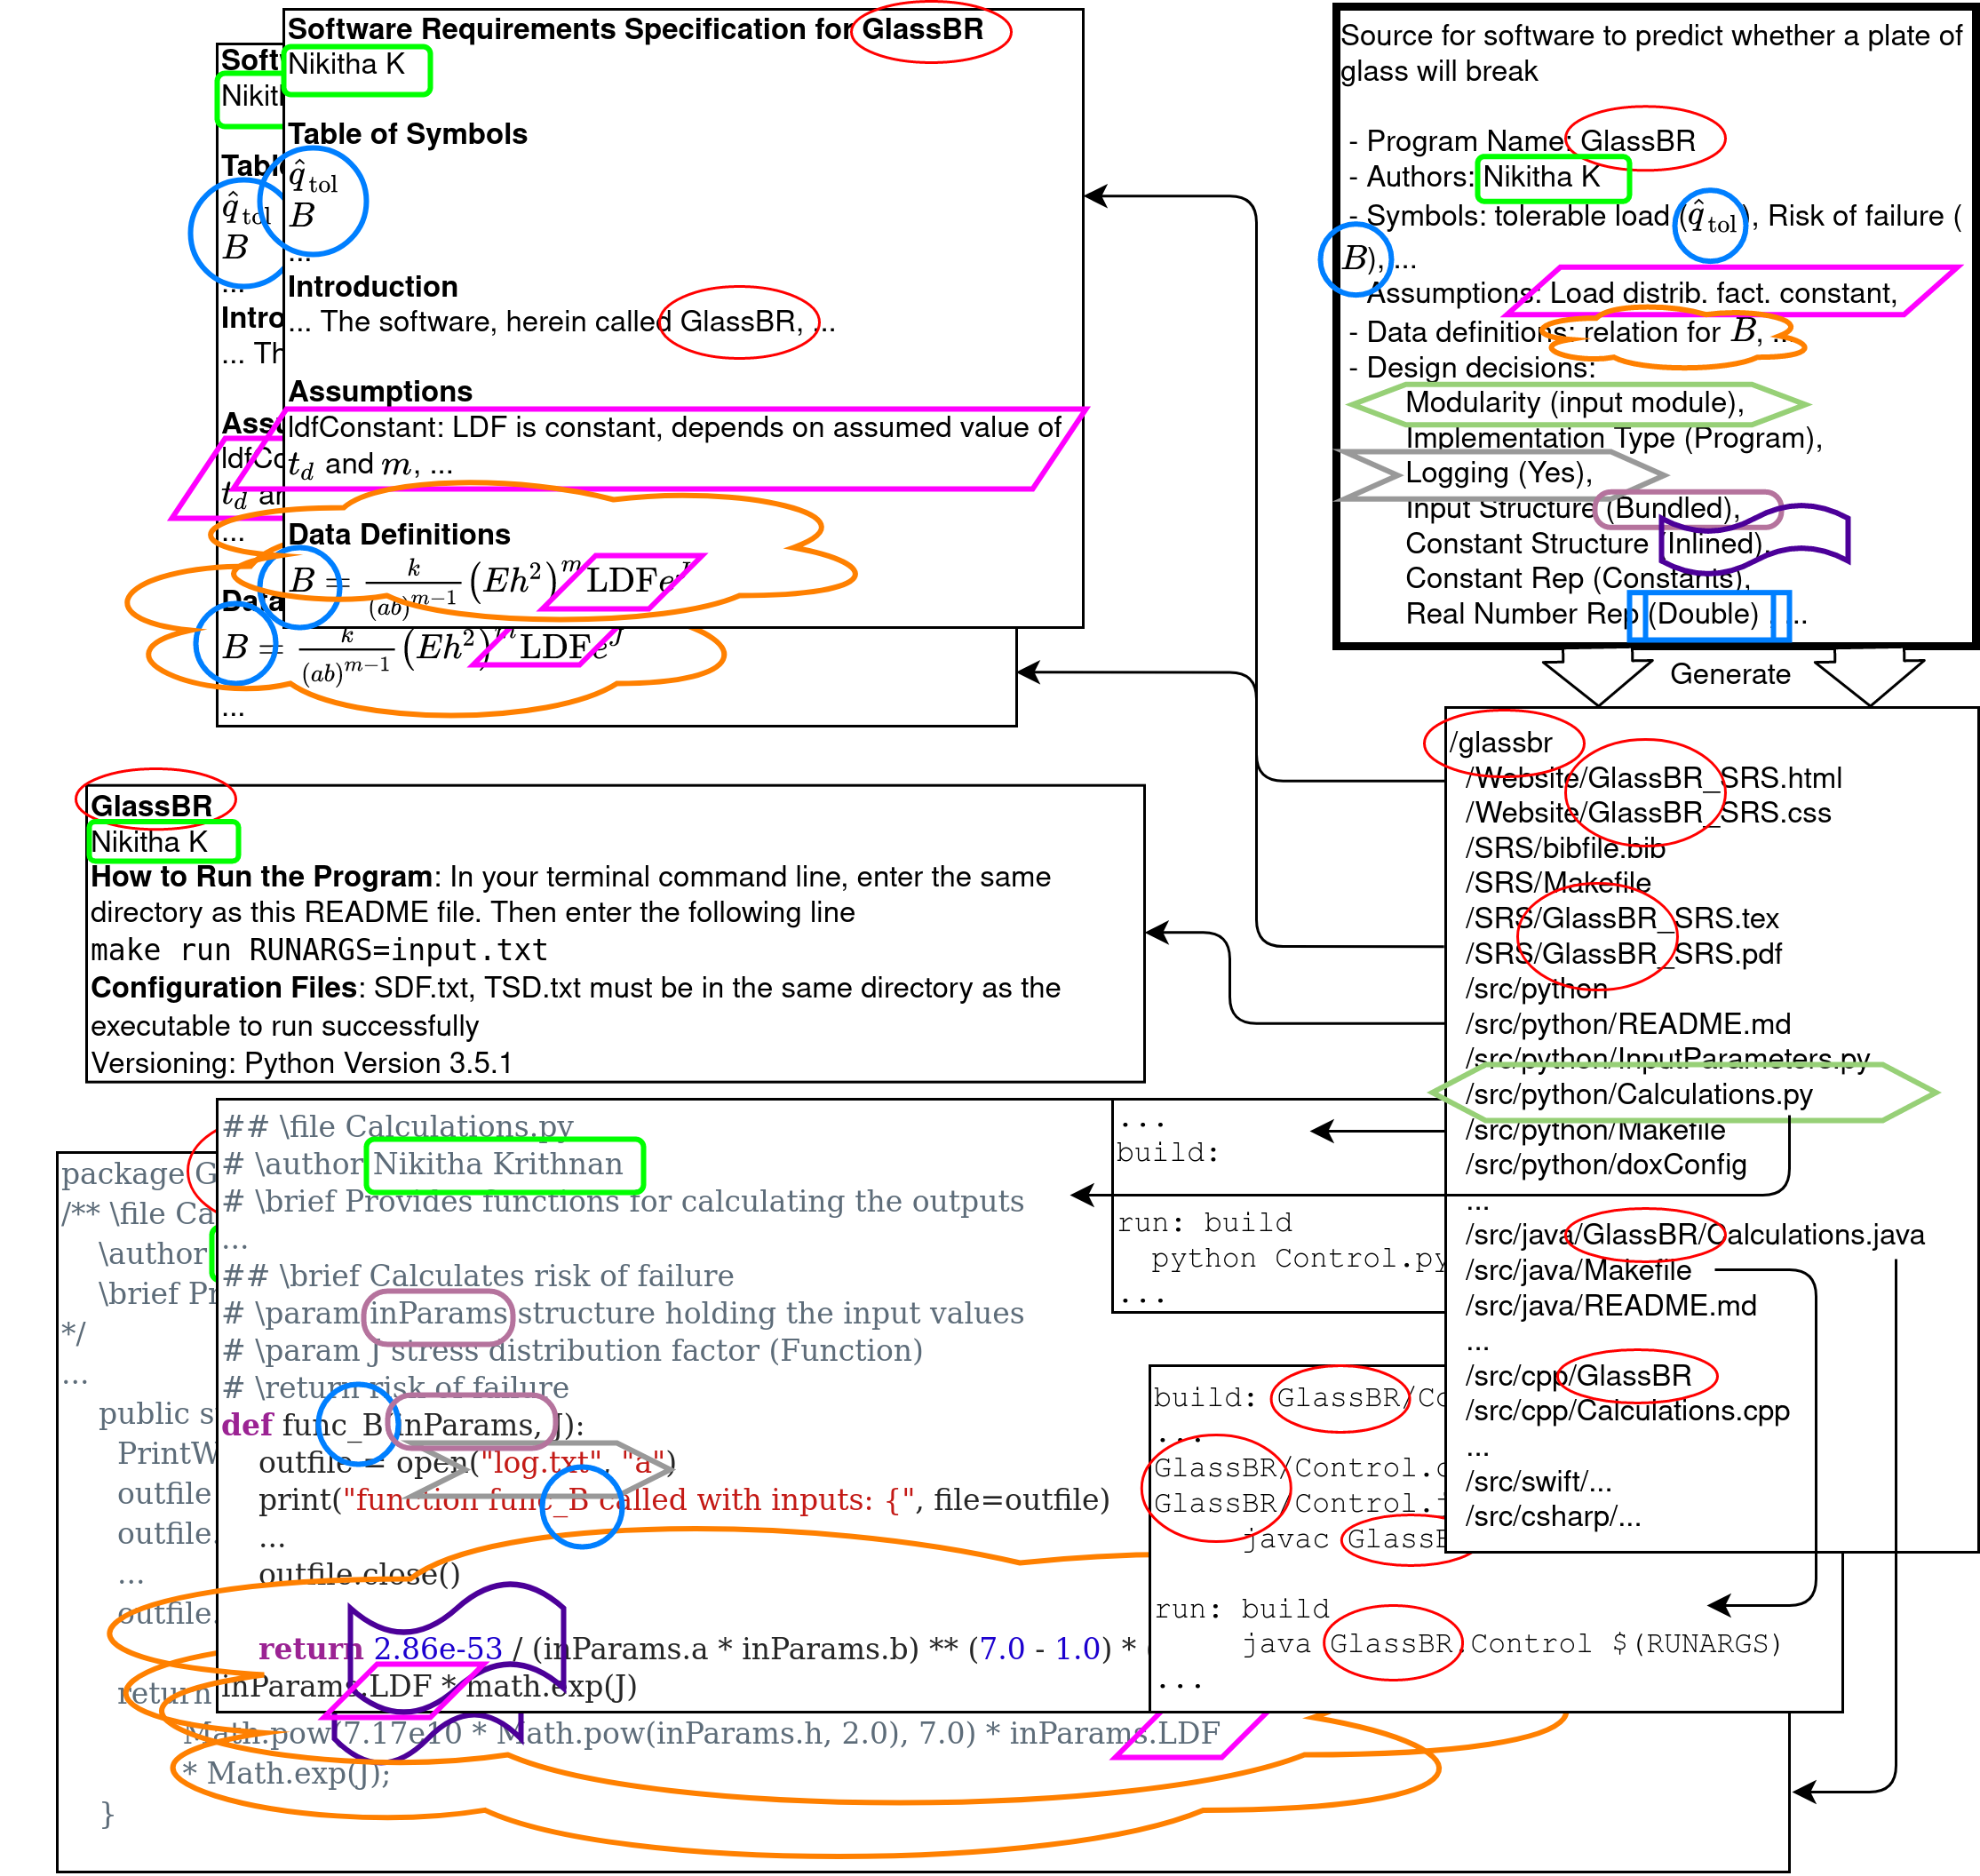
\includegraphics[width=\linewidth]{assets/DrasilSupportsChange-right-portrait-overlapped-ungrouped-11ptFont-squished-blind-v1-300dpi.png}
  \caption{Colors and shapes mapping from captured knowledge to generated
  artifacts.}
  \label{Fig_DrasilAndChange}
\end{figure*}

The transformation of captured knowledge is illustrated in
Figure~\ref{Fig_DrasilAndChange}. This is read starting from the upper right
box. Each piece of information in this figure has its own shape and colour
(orange-cloud, pink lozenge, etc). It should be immediately clear that all
pieces of information reappear in multiple places in the generated artifacts.
For example, the name of the software (GlassBR) ends up appearing more than 80
times in the generated artifacts (in the folder structure, requirements, README,
Makefile and source code). Changing this name would traditionally be extremely
difficult; we can achieve this by modifying a single place, and regenerating.

The first box shows the directory structure of the currently generated
artifacts; continuing clockwise, we see examples of Makefiles for the Java and
Python versions, parts of the fully documented, generated code for the main
computation in those languages, user instructions for running the code, and the
processed \LaTeX{} for the requirements.

The name GlassBR is probably the simplest example of what we mean by
\emph{knowledge}: here, the concept ``program name'' is internally defined, and
its \emph{value} is used throughout. A more complex example is the assumption
that the ``Load Distribution Factor'' (LDF) is constant (pink lozenge). If this
needs to be modified to instead be an input, the generated software will now
have LDF as an input variable.  We also capture design decisions, such as
whether to log all calculations, whether to in-line constants rather than show
them symbolically, etc. The knowledge for GlassBR can also be reused in
different projects.

We now give example conceptual encodings corresponding to steps of the process.

\subparagraph*{Step 1: Task} Compute the probability that a particular pane of
(special) glass will break if an explosive is detonated at a given distance.
This could be in the context of the glass facade for a building.

\subparagraph*{Step 2: Understood} The details are extensively documented
in~\cite{BeasonEtAl1998, ASTM2009, ASTM2015}.

\subparagraph*{Step 3a: Base Knowledge}
A recurring idea is the different types of \texttt{Glass}:
\begin{center}
  \begin{tabular}{|l|l|l|l|}
    \hline
    \textbf{Concept} & \textbf{Term (Name)} & \textbf{Abbrev.} & \textbf{Domain} \\ \hline
    \texttt{fullyT} & Fully Tempered & FT & \texttt{[Glass]} \\ \hline
    \texttt{heatS} & Heat Strengthened & HS & \texttt{[Glass]} \\ \hline
    \texttt{iGlass} & Insulating Glass & IG & \texttt{[Glass]} \\ \hline
    \texttt{lGlass} & Laminated Glass & LG & \texttt{[Glass]} \\ \hline
    \texttt{glassTypeFac} & Glass Type Factor & GTF & \texttt{[Glass]} \\ \hline
  \end{tabular}
\end{center}

\noindent The ``Risk of Failure'' is definable, using the following template for a
\textit{data definition}:
\begin{center}
  \begin{tabular}{|l|l|}
    \hline
    \textbf{Label} & Risk of Failure \\ \hline
%    \textbf{Symbol} & $B$ \\ \hline
%    \textbf{Units} & Unitless \\ \hline
    \textbf{Equation} & \(B = \frac{k}{(ab)^{m-1}}(Eh^2)^m\mathit{LDF}e^J\) \\ \hline
    \textbf{Description} & \vbox{
      \hbox{\strut \(B\) is the Risk of Failure (Unitless)}
      \hbox{\strut \(k\) is the surface flaw parameter (\(\frac{m^{12}}{N^7}\))}
      \hbox{\strut \(a\) \& \(b\) are the plate length \& width (\textit{m})}
      \hbox{\strut \(...\)}
% Do we want to have all of the variables listed? - No - there isn't room
%      \hbox{\strut $m$ is the surface flaw parameter ($\frac{m^{12}}{N^7}$)}
%      \hbox{\strut $E$ is the modulus of elasticity of glass (\textit{Pa})}
%      \hbox{\strut $h$ is the minimum thickness (\textit{m})}
%      \hbox{\strut $LDF$ is the load duration factor (Unitless)}
%      \hbox{\strut $J$ is the stress distribution factor (Unitless)}
    } \\ \hline
    \textbf{Source} & \cite{ASTM2009}, \cite{BeasonEtAl1998} \\ \hline 
% The Campidelli reference was removed because we cannot really cite personal
% communication and not reveal our identities
  \end{tabular}
\end{center}

% explosion - concept chunk
% glass slag - named chunk
% degree - concept chunk
% user input - named chunk
\subparagraph*{Step 3b: Coherent narrative}
The descriptions in GlassBR are produced using an experimental language using
specialized markup for describing relations between knowledge. For example, the
goal of GlassBR (``Predict-Glass-Withstands-Explosion'') is to ``Analyze and
predict whether the \textit{glass slab} under consideration will be able to
withstand the \textbf{explosion} of a certain \textbf{degree} which is
calculated based on \textit{user input}.'', where italicized names are ``named
ideas'', and bold-faced names are ``concept chunks'' (named ideas with a domain
of related ideas). We call this goal a ``concept instance'' (a concept chunk
applied in some way). This language lets us perform various static analyses on
our artifacts.

\subparagraph*{Step 3c: Characteristics of a good solution}
One of our outputs is a probability, which should be checked to be between \(0\)
and \(1\) (code not shown).

\subparagraph*{Step 4: Specialization of theories}
In the GlassBR example, the main specialization is that the thickness parameter
is not free to vary, but must take one of a specific set of values. The
rationale for this specialization is that manufacturers have standardized the
glass thickness they will provide.

The phenomenological nature of the GlassBR example is atypical in this way; most
research software examples involve more significant specialization, such as
partial differential equations to ordinary, elimination of variables, use of
closed-forms instead of implicit equations, and so on.

%% Commenting this out, as it didn't really represent 4b
%
%\heading{Step 4b: Choices}
%
%We create a closed harmonic system containing all related knowledge (in
%particular, the grounded theories), which is as simple as collecting them into a
%single system.
%
%\begin{lstlisting}
%iMods :: [InstanceModel]
%iMods = [pbIsSafe, lrIsSafe]
%
%si :: SystemInformation
%si = SI {
%_sys = glassBR, _kind = Doc.srs, _authors = [nikitha],
%_purpose = purpDoc glassBR Verbose, _quants = symbolsForTable,
%_concepts = [] :: [DefinedQuantityDict], _instModels = iMods,
%_datadefs = GB.dataDefs, _configFiles = configFp,
%_inputs = inputs, _outputs = outputs,
%_defSequence = qDefns, _constraints = constrained,
%_constants = constants, _sysinfodb = symbMap,
%_usedinfodb = usedDB, refdb = refDB
%}
%\end{lstlisting}

\subparagraph*{Step 5: Code-level choices}
We can choose the output programming language, how ``modular'' the generated
code is, whether we want programs or libraries, the level of logging and
comments, etc. Here we show the actual code we use for this, as it is reasonably
direct.


\begin{lstlisting}
code :: CodeSpec
code = codeSpec fullSI choices allMods

choices :: Choices
choices = defaultChoices {
 lang = [Python, Cpp, CSharp, Java, Swift], 
 modularity = Modular Separated,
 impType = Program, logFile = "log.txt", 
 logging = [LogVar, LogFunc],
 comments = [CommentFunc, CommentClass, CommentMod], 
 doxVerbosity = Quiet,
 dates = Hide, 
 onSfwrConstraint = Exception, onPhysConstraint = Exception,
 inputStructure = Bundled, 
 constStructure = Inline, constRepr = Const
}
\end{lstlisting}

\subparagraph*{Step 6: Recipe to generate artifacts}

The various pieces of knowledge specified in the previous steps are assembled
into \emph{recipes} for generating the artifacts, for example specification,
code, dependency diagrams and log of all choices used.  Each one of these has
its own DSL that encodes the parts of a specification, the requirements for
code\footnote{which has been already published and will be cited later}, etc.

The venerable \texttt{Makefile} language is a good example of a DSL for
specifying build scripts, but where our ideas are more properly compared with
the kind of thinking behind \textit{Rattle}~\cite{mitchell:rattle_18_nov_2020}.

And finally, we can put all of these things together, and generate
\textbf{everything}:
\begin{lstlisting}
main :: IO()
main = do
  setLocaleEncoding utf8
  gen (DocSpec (docChoices SRS [HTML, TeX]) "GlassBR_SRS") srs printSetting
  genCode choices code
  genDot fullSI
  genLog fullSI printSetting
\end{lstlisting}

\section{Concluding Remarks}
\label{sec:concluding-remarks}


% To summarize:
% \\

\begin{figure}
  \centering
  \fbox{
    \begin{minipage}[c]{0.65\textwidth}
      \centering
      \begin{tabular}{rcl}
        \textbf{Opportunity} & : & well-understood + long-lived \\
        \textbf{Tools}       & : & knowledge capture + DSLs + generators \\
        \textbf{Result}      & : & \emph{long-term productivity gain}
      \end{tabular}

      % \begin{itemize}%[leftmargin=\widthof{[\textbf{Opportunity}]}]
      %   \item[\textbf{Opportunity}]: well-understood + long-lived
      %   \item[\textbf{Tools}]: knowledge capture + DSLs + generators
      %   \item[\textbf{Result}]: \emph{long-term productivity gain}
      % \end{itemize}
    \end{minipage}
  }
  \caption{Summary}
  \label{fig:summary}
\end{figure}

We get productivity gains because there is in fact an incredible amount of
\emph{knowledge duplication} present in software, especially in well understood
domains. For these domains building software really should be a matter of
assembly-line style engineering. Furthermore, there is also inherent knowledge
duplication between the artifacts of a project because \emph{they are about the
same topic}.

This means that if we spend some up-front time capturing the fundamental
knowledge of specific domains (such as mechanics of rigid body motion, dynamics
of soil, trains, etc), most later development time can be spent on the
\emph{specifics} of the given requirements.

As a side-effect, we obtain traceability and consistency, by construction.
Traceability is illustrated by Figure~\ref{Fig_DrasilAndChange}, which shows we
can track where each of the concepts is used.  An example of consistency is
found in the table of symbols that appears in our generated documentation.  The
list of symbols is not entered by the user; it is automatically constructed from
the base knowledge (Step 3a).

There are further ideas that co-exist smoothly with our framework, most notably
software families and correctness.  Our process will remove human errors from
generating and maintaining documentation, code, test cases and build
environments, since these mundane details are handled by the generator.
Furthermore, our work makes it easy to experiment with ``what if'' scenarios,
which make it easy to explicitly track the ramifications proposed changes.  

With the right up-front investment, we can have sustainable software development
because stable knowledge is separated from local context, which is where most of
the rapidly changing assumptions and requirements reside.

%%
%% Bibliography
%%

%% Please use bibtex, 

\bibliography{References}

\end{document}
